\section*{Configuración del \comillas{Path}(adicional)}
  Cabe resaltar que esta parte de la actividad fue realizada para llamar con mas facilidad los programas desde la terminal, dado que   para poder LLamar un programa desde la misma se tiene que indicar la ubicación de los archivos los cuales se quieren ejecutar si este no se encuentra en la \comillas{variable de entorno} \comillas{path} de windows. Para resolver esto se puede realizar lo siguiente:
  \begin{itemize}
    \item  Referirse a un \comillas{path} explicito, se envía este, ya sea absoluto (desde disco local:... en este caso C:) o relativo (desde donde se \comillas{encuentra} la terminal actualmente).

    \item Configuración de la variable de entorno \comillas{path}.
  \end{itemize}

  El primer método no requiere explicación, solo se debe hacer referencia explicita a la ubicación de los archivos que se quiere llamar cada vez que se requieran (compilador o enlazador respectivamente); El segundo método requiere de la configuración de las variables de estado una sola vez y luego permite referirse al compilador o enlazador de forma directa, sin necesidad de especificar el \comillas{path}, para esto se hace:\\

  Se selecciona inicio -$>$ panel de control -$>$ sistema:

\begin{figure}[H]
  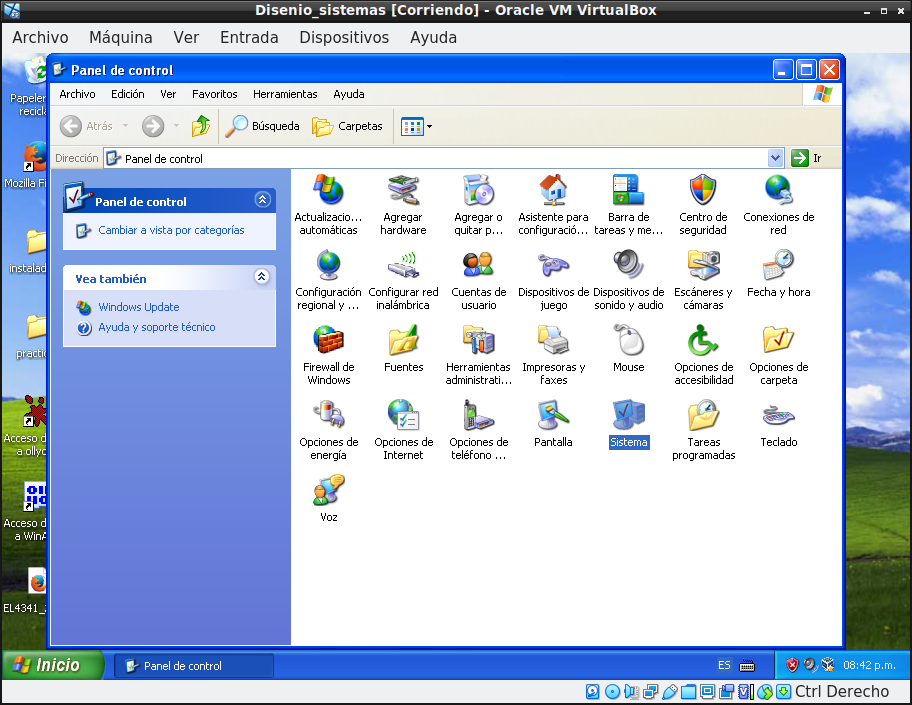
\includegraphics[width=\linewidth]{practica2/imagenes/path/1.png}
  \caption{apertura de ventana sistema}
\end{figure}

  Posteriormente se selecciona, de la ventana emergente de sistema, la opción de variables de entorno y modificar \comillas{path};
  se debe agregar \comillas{;} para indicar un nuevo \comillas{path}, y la dirección explicita de la carpeta. en este caso en particular sería: 
  $C:\backslash masm32 \backslash bin$
\begin{figure}[H]
  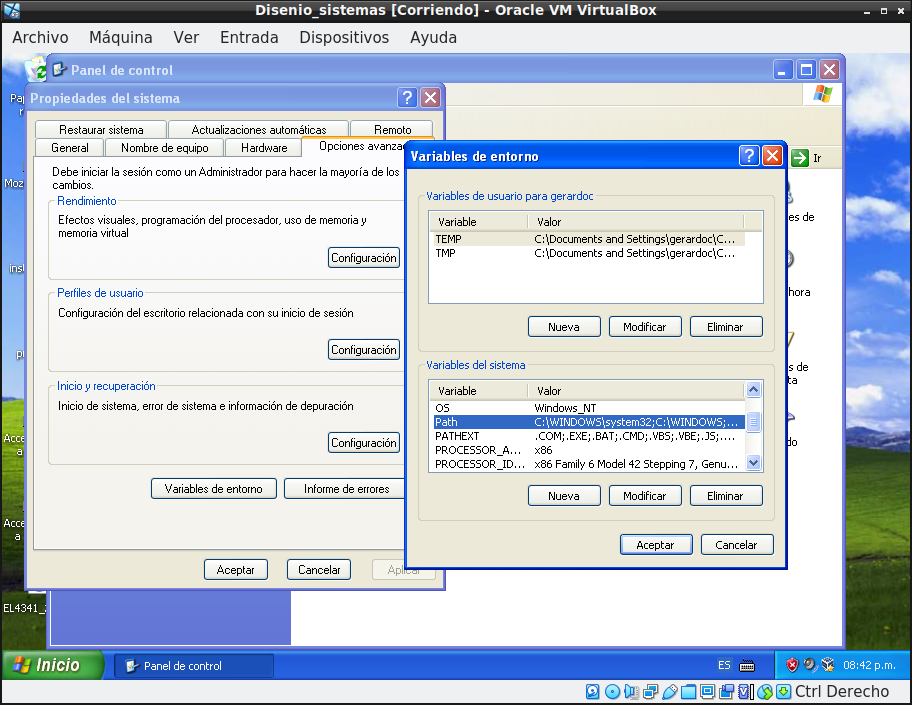
\includegraphics[width=\linewidth]{practica2/imagenes/path/2.png}
  \caption{agregar la variable al path}
\end{figure}



\section{Primera parte}
%\lstinputlisting[language={[x86masm]Assembler}]{hello.asm}

\large{1.3} Ensamble el programa usando la opción Make$>$Assemble.\\
  

\large{1.3.1} para compilar desde la terminal desde el directorio C (se especifican los \comillas{path}) se usa el comando: \\
$\backslash Masm32\backslash Bin\backslash ML \  /c \  /I\comillas{\backslash Masm32\backslash Include}\ $\\
$\comillas{C:\backslash Documents and Settings\backslash gerardoc\backslash Escritorio\backslash practica2\backslash actividad1\backslash act1.asm}$ 

 mas como se incluyo este a las variables de entorno y \comillas{path} general de computadora y ademas se uso el comando cd nueva direccion para moverse entre las carpetas hasta el lugar del archivo act1.asm, se uso el comando: \comillas{$ml \backslash c act1.asm$ }\\


\large{1.3.2} Para este caso particular las únicas opciones (o switches utilizados son:
\begin{itemize}

  \item  /c  el cual le indica a WinASM que solamente debe ensamblar el archivo y no enlazarlo.
  \item /I el cual el programa utiliza automáticamente para ser capaz de incluir el archivo de código fuente \comillas{.asm} que se va a ensamblar.
\end{itemize}



\large{1.3.3} La ventana de salida del WinASM indica la ubicación del ensamblador utilizado, en este caso el \comillas{path} es el siguiente \comillas{$\backslash Masm32\backslash Bin\backslash ML$}. Seguidamente se muestran los switches utilizados, la inclusión del archivo de código fuente.\\
Luego se visualiza la versión del ensamblador utilizado, para este caso el Microsoft (R) Macro Assembler Version 6.14.8444 junto con un mensaje de copyrigth. \\
 Y finalmente indica el resultado del ensamblado, y los errores si existieron.\\



\large{1.3.2} El ensamblador produce un archivo objeto, con formato \comillas{.obj}.\\





\large{1.4} Enlace el programa usando la opción Make$>$Link. Note qué archivo es producido por el enlazador.\\


\large{1.4.1} Con las configuraciones mencionadas anteriormente(\comillas{path} fijado y en la carpeta del archivo, el comando que se utiliza es:  Link16 act1.obj, cabe resaltar que da opciones para:
\begin{itemize}
  \item cambiar el nombre del ejecutable. Da una opción (\comillas{act1.exe} en este caso) por defecto si no se agrega nada.

  \item incluir otros archivos. \comillas{nul.map} por defecto.

  \item Seleccionar el \comillas{path} de las librerías, de nuevo se uso por defecto.

  \item un archivo de definiciones, \comillas{nul.def} por defecto.
\end{itemize}


\large{1.4.2} Ningún switch es utilizado en este apartado\\


\large{1.4.3} Adicional a mostrar los archivos que se ejecutan para realizar el \comillas{linking}, los cuales están en las
siguientes direcciones,
$\comillas{\backslash Masm32\backslash Bin\backslash Link16}$ y $\comillas{C:\backslash WinAsm\backslash link.war} $\\
Se muestra la versión del enlazador utilizado (Microsoft (R) Segmented Executable Linker Version 5.60.339 Dec 5 1994) y el mensaje del copyrigth asociado.begingroup.\\ 
El archivo \comillas{.obj} que se va a enlazar, en este caso \comillas{act1.obj}\\
La finalización o no del proceso y los errores existentes (o ninguno)

\large{1.4.4} El archivo ejecutable del programa \comillas{act1.exe}


\large{1.5}Ejecute el programa usando la opción Make$>$Execute.\\ 

Al ejecutar el archivo, se abre una ventana de \comillas{símbolo del sistema} ubicada en \comillas{path} del archivo ejecutable, en la cual se muestra \comillas{Hello, World!} y al presionar una tecla se cierra



\begin{figure}[H]
  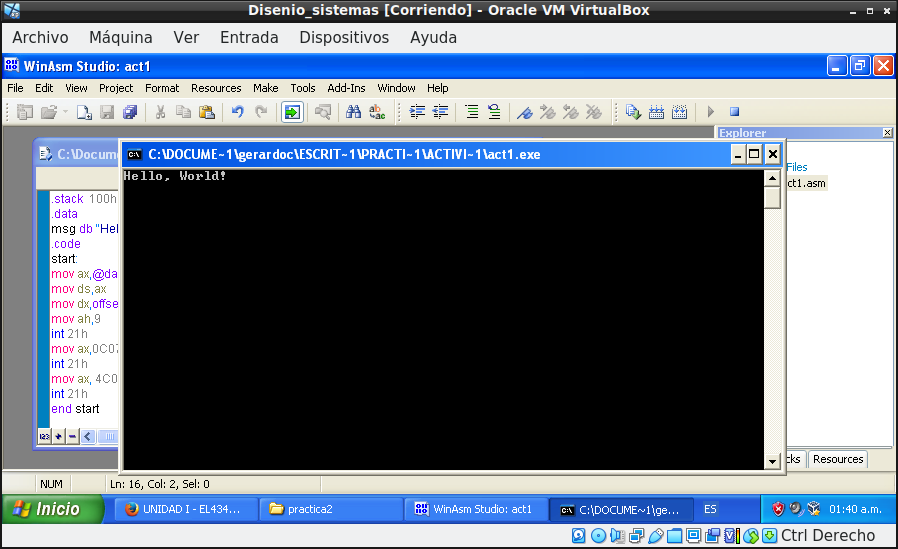
\includegraphics[width=\linewidth]{practica2/imagenes/ej1/ej1.png}
  \caption{programa1 desde WinAsm}
\end{figure}

\begin{figure}[H]
  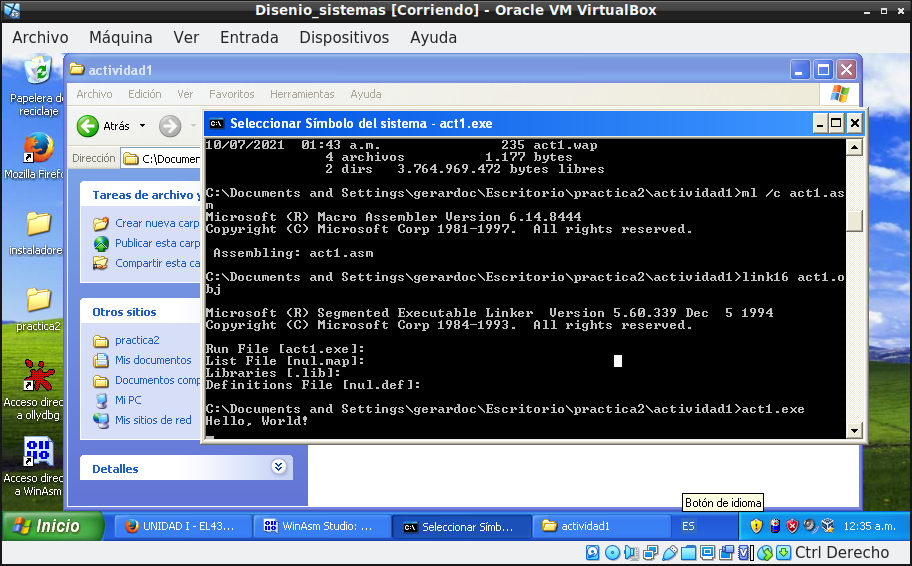
\includegraphics[width=\linewidth]{practica2/imagenes/ej1/ej1terminal.png}
  \caption{programa1 desde terminal}
\end{figure}




\large{1.6} Ejecute el programa por medio de OllyDbg. \\

Al introducir el archivo .exe a Olly, inmediatamente aparece un mensaje que advierte que el
archivo probablemente no es un ejecutable portátil de 32 bits.
Al abrir se muestran las ventanas regulares del Olly, donde se muestra la memoria, instrucciones y valores actuales de los registros, cabe resaltar que es bastante dificil de interpretar. Adicionalmente cuando se procede a correr el programa, se observa que el sistema se detiene automaticamente en la salida de cada llamada, a subsistema o fin definitivo, y por ende hay que precionar varias veces el boton de continuar para ver el mensaje en pantalla.

\begin{figure}[H]
  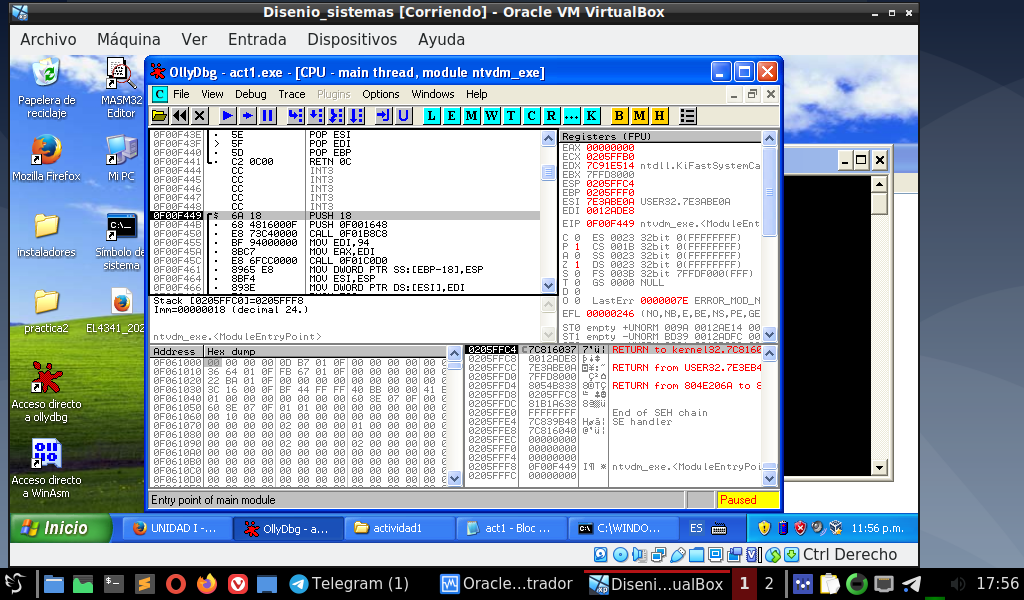
\includegraphics[width=\linewidth]{practica2/imagenes/ej1/olly2.png}
  \caption{programa1 desde Olly inicio}
\end{figure}

\begin{figure}[H]
  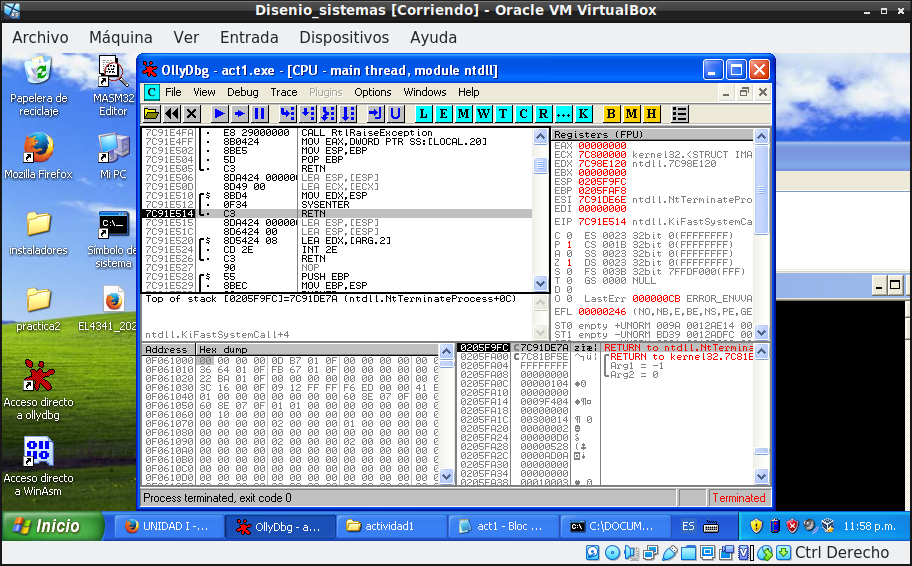
\includegraphics[width=\linewidth]{practica2/imagenes/ej1/olly5.png}
  \caption{programa1 desde Olly fin}
\end{figure}



\section{Segunda parte}

\large{2.3} Ensamble el programa usando la opción Make$>$Assemble.\\

\large{2.3.1} Similarmente para compilar desde la terminal, en el directorio del proyecto se usa el siguiente comando: \\
$ml \  /c \  \comillas{act2.asm}$\\

\large{2.3.2} Para este caso la única opción (o switch utilizado es):
\begin{itemize}
  \item  /c  el cual le indica a MASM que solamente se debe ensamblar el archivo y no enlazarlo.
\end{itemize}

\large{2.3.3} Similar al caso anterior, se muestra que se ensamblo correctamente el archivo, mostrando su nombre.\\


\large{2.3.4} Se produce un unico archivo, act2.obj.\\

\large{2.4} Enlace el programa uando la opción Make$>$Link\\

\large{2.4.1} Para enlazar el programa desde la terminal, se usa el siguiente comando $link16\ act2.obj\ ,,,,,$. Las comas se agregan para evitar que el programa solicite los archivos adiccionales.\\

\large{2.4.2} No se utiliza ningun opcion en la linea de comandos.\\

\large{2.4.3} Ocurre un error, debido a que el programa usa win32 y otras librerias de 32 bits no compatibles con ms-dos.

\begin{figure}[H]
  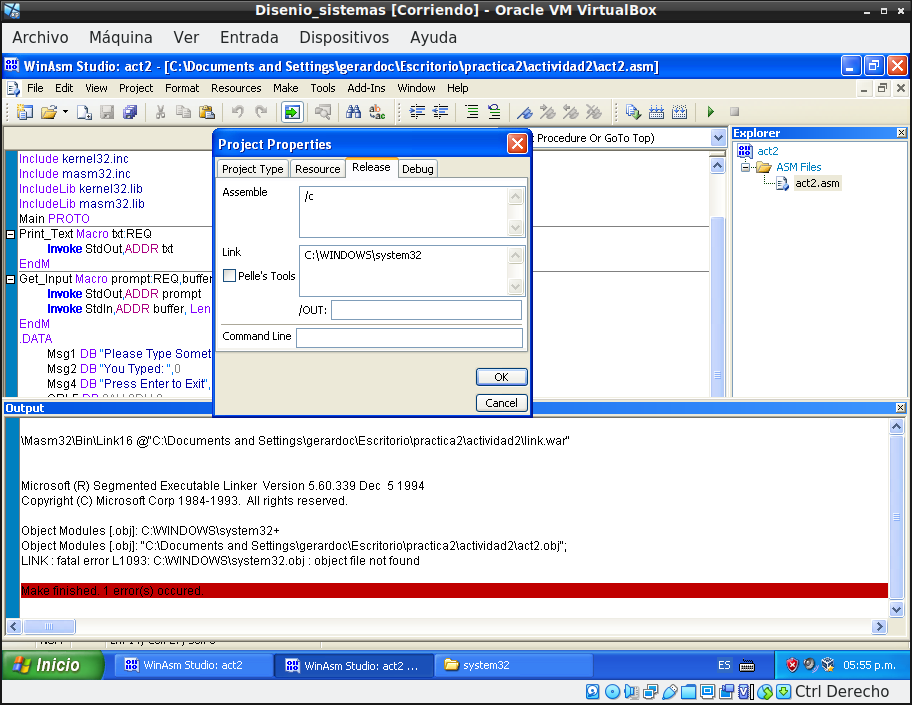
\includegraphics[width=\linewidth]{practica2/imagenes/ej2/ej2_2doerror.png}
  \caption{error programa 2}
\end{figure}

\large{2.4.4} Ninguna, el programa no se pudo enlazar.\\ 

\large{2.5} Como no se creo ningun programa, ejecutar no produce ninguna acción.\\ 

\large{2.6} No existe ningun programa para depurar.\\ 



\section{Tercera parte}
\large{3.3} Ensamble el programa usando la opción Make$>$Assemble.\\

\large{3.3.1} Para compilar desde la terminal, en el directorio del proyecto se usa el siguiente comando: \\
$ml \  /c /coff\  \comillas{act1.asm}$.\\

\large{3.3.2} Las opciones usadas (o switches utilizados) son:
\begin{itemize}
  \item  /c  El cual le indica a MASM que solamente se debe ensamblar el archivo y no enlazarlo.
  \item  /coff Esta Opcion se utiliza para indicar que queremos que el archivo ensamblado sea de tipo coff y no de tipo OMF (usado en 16 bits)
\end{itemize}

\large{3.3.3} Produce un error de ensamblaje, debido a que a el programa no es compatible con la opcion coff. Sin esta opcion no se puede enlazar como aplicacion de consola y esto ocurre porque el programa es de ms-dos y no es compatible con windows NT.

\begin{figure}[H]
  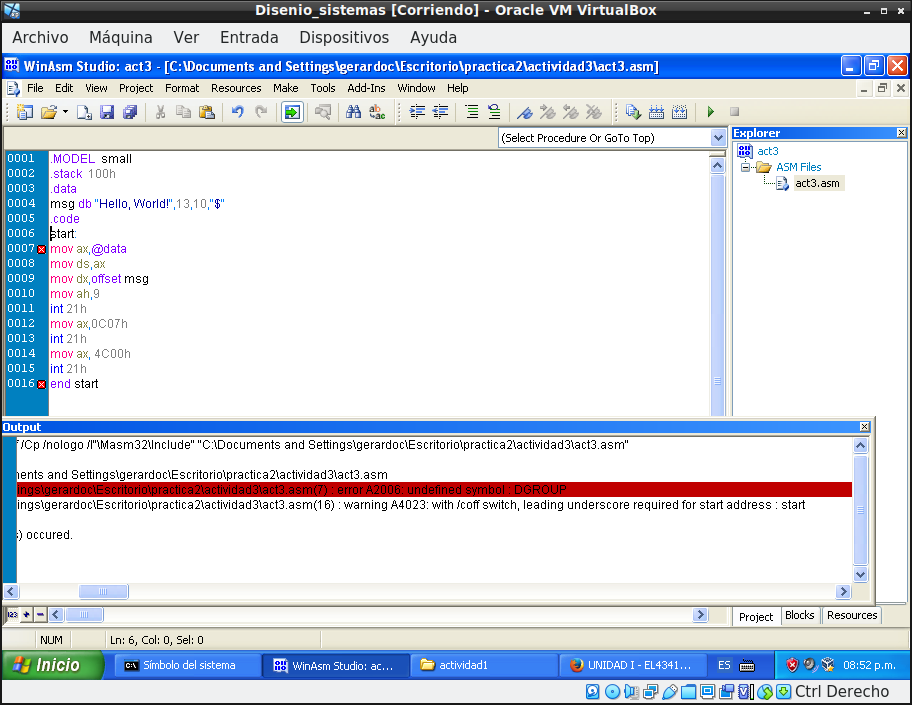
\includegraphics[width=\linewidth]{practica2/imagenes/ej3/error.png}
  \caption{error ensamblaje programa 1}
\end{figure}

\large{3.3.4} No se produce ningun archivo\\

\large{3.4} Enlace el programa uando la opción Make$>$Link\\

\large{3.4.1} Para enlazar el programa desde la terminal, se usaria el siguiente comando $link\ act1.obj\ /SUBSTEM:CONSOLE\ \dots$\\

\large{3.4.2} No se utiliza ningun opcion en la linea de comandos.
Sin embargo, no se pudo ensamblar el programa por lo tanto no se puede enlazar\\

\large{3.4.3} No existe arhcivo para enlazar\\

\large{3.4.4} Ninguna, el programa no se pudo enlazar.\\

\large{3.5} Como no se creo ningun programa, ejecutar no produce ninguna acción.\\

\large{3.6} No existe ningun programa para depurar.\\




\section{Cuarta parte}
\large{4.3} Ensamble el programa usando la opción Make$>$Assemble.\\

\large{4.3.1} se usa el siguiente comando desde la terminal:\\
 $ml \  /c\  /coff\  /Cp\  /nologo\ /I\comillas{\backslash Masm32\backslash Include}\ act4.asm$ \\
 mas, WinAsm usa: \\
 $\backslash Masm32\backslash Bin\backslash ML \  /c\  /coff\  /Cp\  /nologo\ /I\comillas{\backslash Masm32\backslash Include}$\\$ \comillas{C:\backslash Documents and Settings\backslash gerardoc\backslash Escritorio\backslash practica2\backslash actividad4\backslash act4.asm}$\\


\large{4.3.2} los switches usados son: 
\begin{itemize}
 \item /c para indicar que solamente se va a ensamblar.
 \item /coff para generar un archivo objeto de formato .coff .
 \item /Cp para preservar las mayusculas/minusculas de todos los identificadores de usuario, case sensitive.
 \item /nologo  para suprimir los mensajes de ensamblado exitoso.
\end{itemize}


\large{4.3.3} La salida es:
\begin{verbatim}
Assembling: 
C:\Documents and Settings\gerardoc\Escritorio\practica2\actividad4\act4.asm

***********
ASCII build
***********


Make finished. 0 error(s) occured.


\end{verbatim}

la cual, como se observa no da informacion adicional a la explicada anteriormente\\


\large{4.3.4} El archivo generado es act4.obj, un archivo de tipo objeto\\


\large{4.4} Enlace el programa usando la opción Make$>$Link.


\large{4.4.1} El comando usado fue:
\begin{verbatim}
Link /SUBSYSTEM:CONSOLE /RELEASE /VERSION:4.0 "/LIBPATH:\Masm32\Lib"
"C:\Documents and Settings\gerardoc\Escritorio\practica2\actividad4\act4.obj" 
"/OUT:C:\Documents and Settings\gerardoc\Escritorio\practica2\actividad4\act4.exe" 

\end{verbatim}



\large{4.4.2} Los switches utilizados fueron:
\begin{itemize}
  \item /SUBSYSTEM:CONSOLE: Para indicarle al Sistema operativo que debe correr el .exe con la consola
  \item /RELEASE: Para fijar el ‘checksum’ de la cabecera del .exe
  \item /VERSION:4.0: Para asignarle una versión
\end{itemize}


\large{4.4.3} La salida es:

\begin{verbatim}
\Masm32\Bin\Link 
@"C:\Documents and Settings\gerardoc\Escritorio\practica2\actividad4\link.war"

Microsoft (R) Incremental Linker Version 5.12.8078
Copyright (C) Microsoft Corp 1992-1998. All rights reserved.

/SUBSYSTEM:CONSOLE /RELEASE /VERSION:4.0 "/LIBPATH:\Masm32\Lib" 
"C:\Documents and Settings\gerardoc\Escritorio\practica2\actividad4\act4.obj" 
"/OUT:C:\Documents and Settings\gerardoc\Escritorio\practica2\actividad4\act4.exe" 

Make finished. 0 error(s) occured.

\end{verbatim}
que no es mas que el comando, mensaje de copyright y finalizacion exitosa


\large{4.4.4} Genera el archivo ejecutable act4.exe

\large{4.5} Al ejecutar el programa, se abre una ventana de consola de Windows, la cual muestra “Please type something: “. El programa en este punto espera una entrada de texto del usuario, al ser introducida y presionada la tecla enter, el programa muestra “You typed: “y a continuación se muestra el texto escrito en el paso anterior. Luego de esto, la consola permanece mostrando esos mensajes hasta que se presione enter para cerrar la ventana.

desde WinAsm:
\begin{figure}[H]
  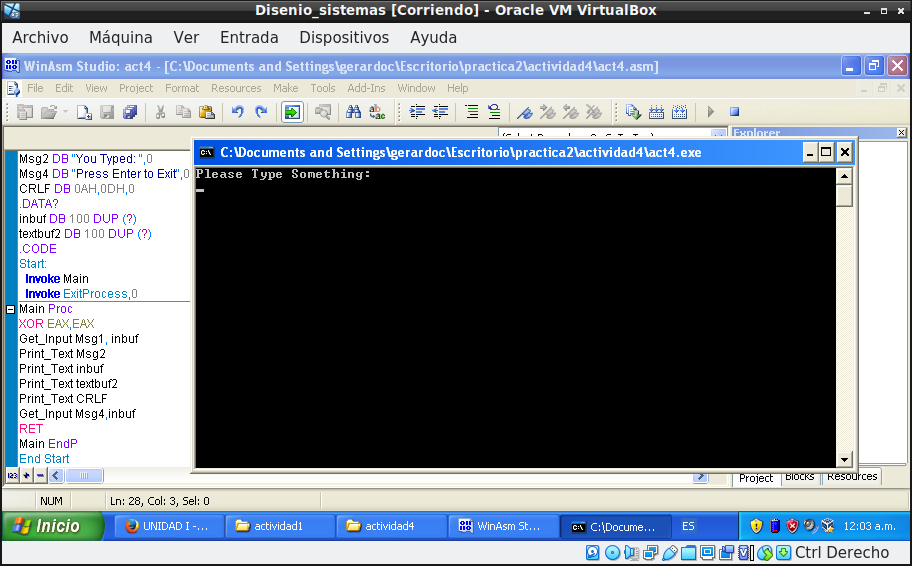
\includegraphics[width=\linewidth]{practica2/imagenes/ej4/ej4a.png}
  \caption{parte 1: programa 4 desde WinAsm}
\end{figure}

\begin{figure}[H]
  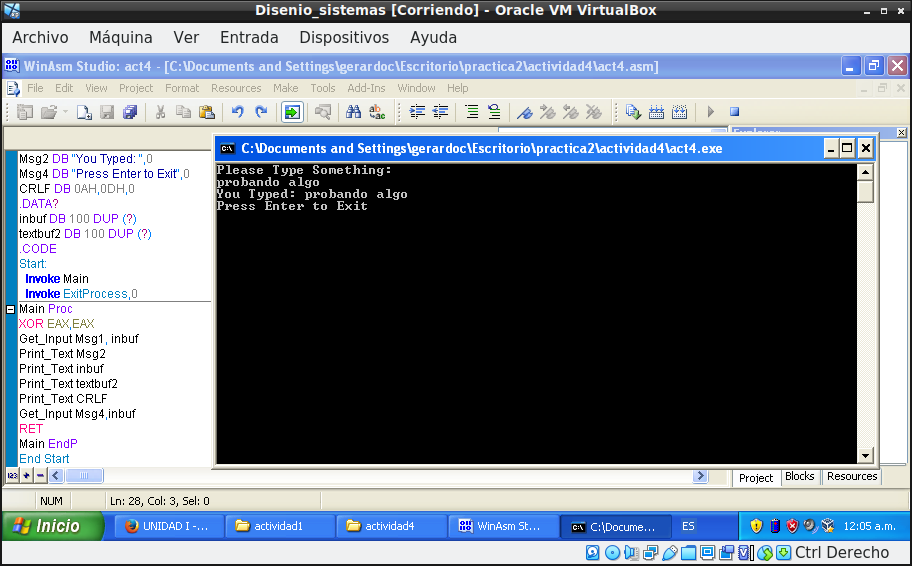
\includegraphics[width=\linewidth]{practica2/imagenes/ej4/ej4b.png}
  \caption{parte 2: programa 4 desde WinAsm}
\end{figure}

desde la terminal: 
\begin{figure}[H]
  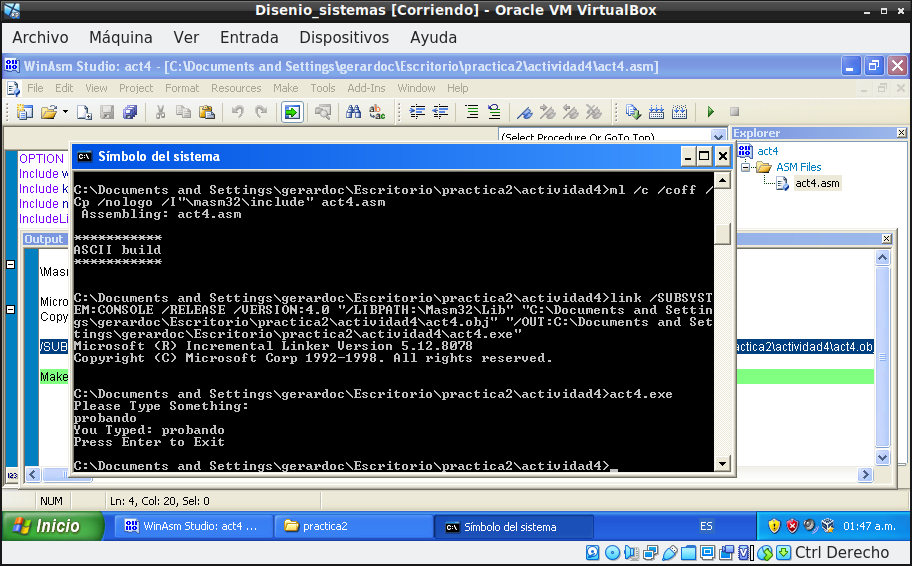
\includegraphics[width=\linewidth]{practica2/imagenes/ej4/ej4_uzcategui_terminal.png}
  \caption{programa 4 desde la terminal}
\end{figure}


\large{4.6} Este programa es un poco mas entendible, y si se ejecuta sin breakpoints solo se detiene para esperar las entradas de usuario.
\begin{figure}[H]
  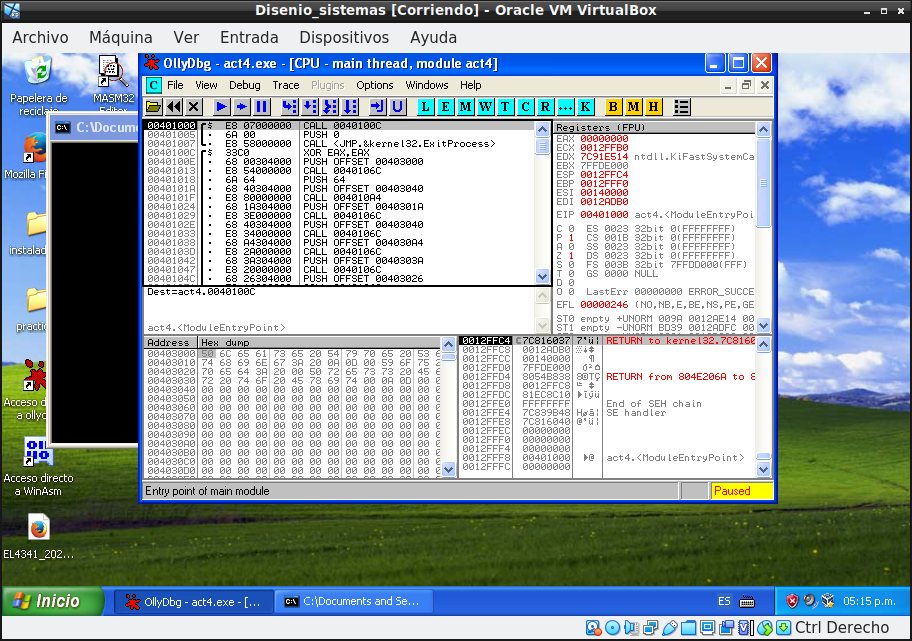
\includegraphics[width=\linewidth]{practica2/imagenes/ej4/olly_ej4.png}
  \caption{programa 4 desde Olly}
\end{figure}


\section{Conclusiones}
1) Ambas aplicaciones funcionan mediante una interfaz de texto, ambas tienen el concepto de standard input y standard ouput, y ambas aplicaciones intereactuan con el sistema operativo mediante APIs de bajo nivel. Sin embargo, las aplicaciones de ms-dos se comunican con el sistema operativo mediante interrupciones, mientras que las de consola cuenta con el API win32; Las aplicaciones de ms-dos son de 16 bits, mientras que las de consola son de 32 bits y la diferencia mas importante es que las aplicaciones de ms-dos son una emulacion sobre una maquina virtual, debido a que a partir de windows xp se usa el nucleo Windows NT, por lo tanto ambos tipos de aplicaciones funcionan con nucleos diferentes.


2) Las aplicaciones de consola pueden parecer una reliquia del pasado, sin embargo son una forma eficiente de comunicarse con aplicaciones para usuarios mas avanzados con el uso de un ordernador y han estado ganando popularidad en los ultimos años. En el caso particular de compilar programas de ensamblador, la terminal es una forma eficiente de compilar proyectos cuando se conocen todas las opciones del ensamblador, ademas de permitir automatizar la construccion de proyectos con el uso de programas de batch.